%%%%%%%%%%%%%%%%%%%%%%%%%%%%%%%%%%%%%%%%%%%%%%%%%%%%%%%%%%%%%%%%%%%%%%%%%%%%%%%%
%
% Template license:
% CC BY-NC-SA 3.0 (http://creativecommons.org/licenses/by-nc-sa/3.0/)
%
%%%%%%%%%%%%%%%%%%%%%%%%%%%%%%%%%%%%%%%%%%%%%%%%%%%%%%%%%%%%%%%%%%%%%%%%%%%%%%%%

%----------------------------------------------------------------------------------------
%	PACKAGES AND OTHER DOCUMENT CONFIGURATIONS
%----------------------------------------------------------------------------------------

\documentclass[
11pt, % The default document font size, options: 10pt, 11pt, 12pt
%oneside, % Two side (alternating margins) for binding by default, uncomment to switch to one side
%chapterinoneline,% Have the chapter title next to the number in one single line
spanish,
singlespacing, % Single line spacing, alternatives: onehalfspacing or doublespacing
%draft, % Uncomment to enable draft mode (no pictures, no links, overfull hboxes indicated)
%nolistspacing, % If the document is onehalfspacing or doublespacing, uncomment this to set spacing in lists to single
%liststotoc, % Uncomment to add the list of figures/tables/etc to the table of contents
%toctotoc, % Uncomment to add the main table of contents to the table of contents
parskip, % Uncomment to add space between paragraphs
%codirector, % Uncomment to add a codirector to the title page
headsepline, % Uncomment to get a line under the header
]{MastersDoctoralThesis} % The class file specifying the document structure

%----------------------------------------------------------------------------------------
%	INFORMACIÓN DE LA MEMORIA
%----------------------------------------------------------------------------------------

\thesistitle{Modelo de inteligencia artificial para la regulación de temperatura en equipos de inducción de hipotermia} % El títulos de la memoria, se usa en la carátula y se puede usar el cualquier lugar del documento con el comando \ttitle

% Nombre del posgrado, se usa en la carátula y se puede usar el cualquier lugar del documento con el comando \degreename
\posgrado{Carrera de Especialización en Inteligencia Artificial} 
%\posgrado{Carrera de Especialización en Internet de las Cosas} 
%\posgrado{Carrera de Especialización en Intelegencia Artificial}
%\posgrado{Maestría en Sistemas Embebidos} 
%\posgrado{Maestría en Internet de las cosas}

\author{Ing. Ezequiel Fernandez} % Tu nombre, se usa en la carátula y se puede usar el cualquier lugar del documento con el comando \authorname

\director{Dr. Lic. Tobías Canavesi (FIUBA)} % El nombre del director, se usa en la carátula y se puede usar el cualquier lugar del documento con el comando \dirname
\codirector{Nombre del codirector (pertenencia)} % El nombre del codirector si lo hubiera, se usa en la carátula y se puede usar el cualquier lugar del documento con el comando \codirname.  Para activar este campo se debe descomentar la opción "codirector" en el comando \documentclass, línea 23.

\juradoUNO{Nombre del jurado 1 (pertenencia)} % Nombre y pertenencia del un jurado se usa en la carátula y se puede usar el cualquier lugar del documento con el comando \jur1name
\juradoDOS{Nombre del jurado 2 (pertenencia)} % Nombre y pertenencia del un jurado se usa en la carátula y se puede usar el cualquier lugar del documento con el comando \jur2name
\juradoTRES{Nombre del jurado 3 (pertenencia)} % Nombre y pertenencia del un jurado se usa en la carátula y se puede usar el cualquier lugar del documento con el comando \jur3name

%\ciudad{Ciudad Autónoma de Buenos Aires}
\ciudad{Ciudad Autónoma de Buenos Aires}

\fechaINICIO{octubre de 2024}
\fechaFINAL{abril de 2025}


\keywords{Sistemas embebidos, FIUBA} % Keywords for your thesis, print it elsewhere with \keywordnames


\begin{document}


\frontmatter % Use roman page numbering style (i, ii, iii, iv...) for the pre-content pages

\pagestyle{plain} % Default to the plain heading style until the thesis style is called for the body content


%----------------------------------------------------------------------------------------
%	RESUMEN - ABSTRACT 
%----------------------------------------------------------------------------------------

\begin{abstract}
\addchaptertocentry{\abstractname} % Add the abstract to the table of contents
%
%The Thesis Abstract is written here (and usually kept to just this page). The page is kept centered vertically so can expand into the blank space above the title too\ldots
\centering

En la presente memoria se describe el diseño e implementación de un modelo de inteligencia artificial para la empresa Amrra Electromedicina, en el marco del programa de vinculación. El objetivo del trabajo fue construir un modelo para regular la temperatura en un sistema de inducción de hipotermia y compararlo con el algoritmo que funciona actualmente en los equipos.
Para el desarrollo fue fundamental la incorporación de los conocimientos adquiridos en la carrera, tales como análisis y preprocesamiento de datos, algoritmos de inteligencia artificial, arquitecturas de aprendizaje profundo y programación en Python.

\end{abstract}

%----------------------------------------------------------------------------------------
%	CONTENIDO DE LA MEMORIA  - AGRADECIMIENTOS
%----------------------------------------------------------------------------------------

\begin{acknowledgements}
%\addchaptertocentry{\acknowledgementname} % Descomentando esta línea se puede agregar los agradecimientos al índice
\vspace{1.5cm}

Esta sección es para agradecimientos personales y es totalmente \textbf{OPCIONAL}.  

\end{acknowledgements}

%----------------------------------------------------------------------------------------
%	LISTA DE CONTENIDOS/FIGURAS/TABLAS
%----------------------------------------------------------------------------------------

\tableofcontents % Prints the main table of contents

\listoffigures % Prints the list of figures

\listoftables % Prints the list of tables


%----------------------------------------------------------------------------------------
%	CONTENIDO DE LA MEMORIA  - DEDICATORIA
%----------------------------------------------------------------------------------------

\dedicatory{\textbf{Dedicado a... [OPCIONAL]}}  % escribir acá si se desea una dedicatoria

%----------------------------------------------------------------------------------------
%	CONTENIDO DE LA MEMORIA  - CAPÍTULOS
%----------------------------------------------------------------------------------------

\mainmatter % Begin numeric (1,2,3...) page numbering

\pagestyle{thesis} % Return the page headers back to the "thesis" style

% Incluir los capítulos como archivos separados desde la carpeta Chapters

% Chapter 1

\chapter{Introducción general} % Main chapter title

En este capítulo se presentan conceptos básicos sobre la temática. También se comenta el contexto y las motivaciones que impulsan la realización de este proyecto. Además se menciona el alcance y los objetivos, y se analiza el estado del arte en el campo de estudio.

\label{Chapter1} % For referencing the chapter elsewhere, use \ref{Chapter1} 
\label{IntroGeneral}

%----------------------------------------------------------------------------------------

% Define some commands to keep the formatting separated from the content 
\newcommand{\keyword}[1]{\textbf{#1}}
\newcommand{\tabhead}[1]{\textbf{#1}}
\newcommand{\code}[1]{\texttt{#1}}
\newcommand{\file}[1]{\texttt{\bfseries#1}}
\newcommand{\option}[1]{\texttt{\itshape#1}}
\newcommand{\grados}{$^{\circ}$}

%----------------------------------------------------------------------------------------

%\section{Introducción}

%----------------------------------------------------------------------------------------
\section{Introducción}

El objetivo de este proyecto es desarrollar un modelo de inteligencia artificial prototipo que estime la temperatura del agua que circula en un equipo utilizado para la inducción de hipotermia a pacientes neonatales. Además se hará foco en la incidencia de los parámetros que se disponen en el cálculo para aportar al conocimiento sobre estos tratamientos. Esto puede significar a futuro una mejora en un producto que desarrolla la empresa y brindar a quienes necesiten este tratamiento un desarrollo superador del mismo respecto a la actualidad. El proyecto será desarrollado dentro del marco del programa de vinculación. 

La empresa es AmrrA y los equipos en cuestión tienen el nombre Amrraterm HTF. Estos sistemas se utilizan con el propósito de inducir una hipotermia controlada en pacientes neonatales. Existen contextos en los cuales esto proporciona una mejor evolución de los pacientes. El principal caso de uso es el de pacientes que sufren hipoxia al nacer, esto es, falta de oxígeno en el cerebro. En estos casos, a temperatura corporal normal la interacción entre las neuronas es alta y se pueden desarrollar efectos adversos en la capacidad cerebral del paciente. Por esto un tratamiento estándar es el de inducir hipotermia por 72 horas a fin de minimizar los efectos que la hipoxia puede generar a futuro en los pacientes. 

Para lograr esto el procedimiento estándar es sedar al paciente y colocarlo dentro de una incubadora, donde es envuelto en las mantas que forman parte del equipo. Por estas mantas circula agua destilada. El equipo recibe como dato de entrada la temperatura objetivo a la cual se quiere llevar al paciente, que suele ser de 33,5º C, y regula la temperatura del agua en función de la temperatura objetivo y la actual del paciente. Una vez terminado el tratamiento de hipotermia, el equipo funciona en un modo llamado rampa, en el cual sube paulatinamente la temperatura hasta llegar a un estado normal.

En la actualidad la temperatura del agua es regulada por un algoritmo de lógica difusa. En un rango de pesos estándar de los pacientes (entre 2,5 kg y 3,5 kg) el algoritmo funciona correctamente, pero es posible que en pesos inferiores o superiores haya comportamientos que este proyecto pueda mejorar. Se desarrollará este modelo para evaluar si funciona mejor que el algoritmo actual en ese rango, en los valores inferiores o en los superiores de peso. 

Se utilizarán diversos datos para construir un modelo acorde al problema como el peso del paciente, la edad, la temperatura objetivo y las variaciones de temperatura del agua y paciente. Además de construir un modelo superador, también se busca detectar la incidencia de ciertos parámetros, como el peso del paciente, que no se utiliza por el algoritmo actual. Para evaluar el comportamiento del modelo se implementa un entorno que permita ingresar datos y visualizar la respuesta del modelo para los datos ingresados. 

El equipo consta de una interfaz mediante la cual el personal de salud indica los datos necesarios, un sistema de mantas y cañerías por las que circula agua destilada,  un sistema térmico con la responsabilidad de administrar la energía para que el agua esté a la temperatura indicada y un algoritmo de lógica difusa responsable de calcular la temperatura óptima del agua para el tratamiento. Un diagrama de esto se puede apreciar en la figura \ref{fig:actual-diagram}. 

\vspace{1cm}

\begin{figure}[htbp]
	\centering
	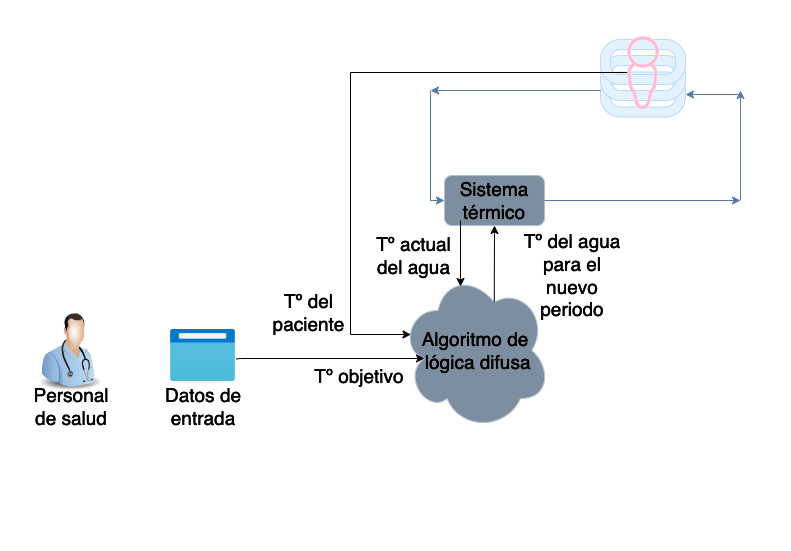
\includegraphics[width=1\textwidth]{./Figures/actual.png}
	\caption{Diagrama de funcionamiento del equipo.}
	\label{fig:actual-diagram}
\end{figure}

\vspace{1cm}

El modelo implementado cumple el mismo rol que el algoritmo que funciona actualmente, por lo que en el diagrama se lo puede ubicar a la par. Además de la temperatura objetivo, la actual del agua y la actual del paciente, recibirá el peso del paciente, y se compara el comportamiento de ambas soluciones. Se propone que funcionen un tiempo en paralelo y un elector defina cual de las temperaturas elegidas aplicar. Un diagrama de esto se puede apreciar en la figura \ref{fig:model-diagram}. 

\vspace{1cm}

\begin{figure}[htbp]
	\centering
	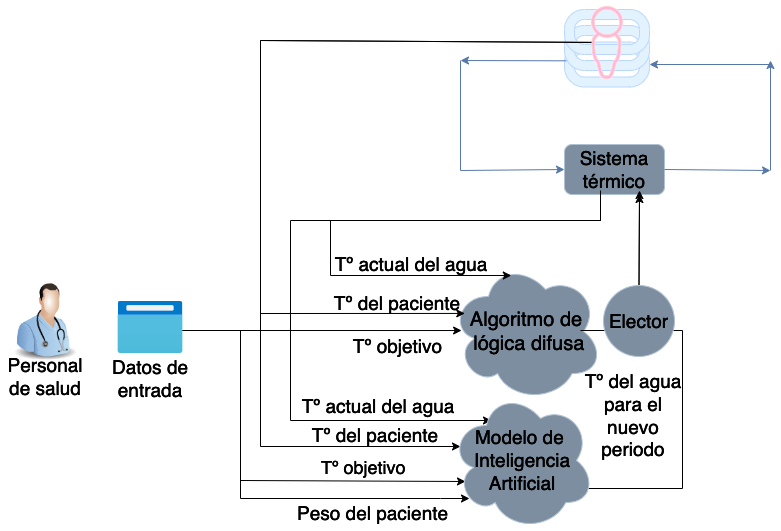
\includegraphics[width=1\textwidth]{./Figures/modelo.png}
	\caption{Diagrama del equipo con el nuevo modelo.}
	\label{fig:model-diagram}
\end{figure}

\vspace{1cm}

\section{Motivación}

Existen dos motivaciones fundamentales para el desarrollo de este proyecto. Por un lado, esta la incorporación de técnicas de inteligencia artificial para el modelado de tratamientos de inducción de hipotermia en los equipos mencionados, lo que supone una actualización al modelado actual y se puede esperar un comportamiento superador, lo que implicaría una mejor evolución en los pacientes. Por el otro, esta la incorporación del peso como variable para modelar el problema, lo que supone un mejor comportamiento y nuevamente, una mejoría en la evolución de los pacientes.
Sin embargo, es posible que el modelo resultante no se comporte mejor que el algoritmo actual. Estos equipos están en funcionamiento en una gran cantidad de hospitales en todo el país, y su funcionamiento es aceptado por la comunidad médica. En este caso, igual este proyecto aportará valor a la empresa, ya que brindará información acerca de la incidencia de los parámetros, y esto brindará un crecimiento en el conocimiento que se tiene sobre estos tratamientos.


\section{Conceptos generales}
A continuación mencionaremos la definición de algunos conceptos y valores importantes para la temática.
Como se mencionó anteriormente, los equipos en cuestión se denominan Amrraterm HTF. Algunos son propiedad de la empresa y se alquilan en centros de salud, mientras que otros fueron adquiridos. Están en funcionamiento en hospitales públicos y privados. Su dominio es acotado al tratamiento de regulación de temperatura en pacientes neonatales, esto es, en recién nacidos. El principal caso de uso es el de provocar una hipotermia controlada en pacientes que sufren hipoxia al nacer. Para esto, el profesional establece una temperatura a la que quiere llevar al paciente. Esta temperatura la denominamos temperatura objetivo. 
Los tratamientos suelen durar 72 hs. aproximadamente. Existen tres etapas en este tiempo. La primera, llamada rampa hacia abajo, se da en los primeros minutos del tratamiento, periodo en el que se busca llevar la temperatura del paciente hacia la objetivo, producto de la circulación de agua fría por las mantas. En la segunda etapa prima la estabilidad, aquí el objetivo es mantener al paciente en la temperatura objetivo. En la última etapa, denominada rampa hacia arriba, producto de la circulación de agua con mayor temperatura en las mantas del equipo, el paciente recupera su temperatura normal.
Al establecer los parámetros del tratamiento, el profesional indica el peso del paciente. Este dato no es tenido en cuenta por el algoritmo actual pero si se utiliza para el entrenamiento de los modelos de este proyecto.
Los pacientes suelen estar en un peso superior a 2,5 kg e inferior a 3,5 kg. En porcentaje, el desvío de este valor no es despreciable.

Podemos distinguir los siguientes atributos:
\begin{itemize}
	\item Temperatura objetivo, a la que se quiere llevar al paciente.
	\item Temperatura del agua que circula por las mantas.
	\item Temperatura actual del paciente en un instante del tiempo.
	\item Peso del paciente.
\end{itemize}

Uno de los criterios de bondad de estos equipos es que, en la etapa estable, la temperatura del paciente diste lo mínimo de la temperatura objetivo. En la práctica se ve que la temperatura oscila sobre la temperatura objetivo, por lo que podemos decir que un modelo será mejor que el actual, en la etapa estable, si la amplitud de la oscilación sobre la temperatura objetivo es menor.

\section{Objetivos y alcance}
Para el presente proyecto se plantean objetivos funcionales y conceptuales. Desde el punto de vista funcional se busca el desarrollo de una solución de inteligencia artificial acorde al problema planteado, lo que significa un nuevo enfoque respecto a lo que utilizan actualmente, una actualización y una potencial mejora de su producto. Desde el lado conceptual, se busca entender la incidencia de los parámetros, con mayor énfasis en el peso y en el comportamiento del modelo respecto a pacientes de distinto peso.

Se definieron los siguientes requerimientos:

\begin{enumerate}
	\item Requerimientos funcionales:
	\begin{enumerate}
		\item El modelo debe predecir el cambio de temperatura óptimo a aplicar.
		\item La salida del modelo debe ser conceptualmente análoga a la del algoritmo de lógica difusa utilizado actualmente, a fin de poder compararlos.
		\item El modelo debe dar una respuesta en un tiempo promedio menor o igual a 10 veces el tiempo promedio de respuesta del algoritmo actual.
		\item El sistema debe permitir ingresar datos de forma manual y mostrar el resultado.
		\item Se debe calcular la incidencia del peso y de los demás atributos en la solución.
	\end{enumerate}
	\item Requerimientos conceptuales:
	\begin{enumerate}
		\item Deben utilizarse datos sintéticos en las pruebas.
	\end{enumerate}
	\item Requerimiento de testing:
	\begin{enumerate}
		\item Se deben ejecutar pruebas secuenciales con datos reales y mostrar una comparación entre los resultados del modelo a implementar y del algoritmo actual.
		\item Se deben comparar tiempos entre el modelo propuesto y el algoritmo actual.
		\item Se debe calcular una métrica a definir para calcular la performance del modelo.
	\end{enumerate}
	\item Requerimiento de documentación:
	\begin{enumerate}
		\item Se deben documentar las decisiones tomadas.
		\item Se deben documentar los resultados de las pruebas y las distintas métricas.
		\item Se requiere documentar el código y las formas de utilizar al sistema.
	\end{enumerate}
	\item Requerimiento asociados con regulaciones
	\begin{enumerate}
		\item Se requiere que los casos utilizados no expongan datos que infrinjan derechos de privacidad.
	\end{enumerate}
\end{enumerate}


El proyecto no incluye: 
\begin{itemize}
	\item La incorporación del modelo a los equipos en funcionamiento.
	\item El despliegue del modelo en la nube.
	\item El desarrollo de una interfaz gráfica, una aplicación o una web.
\end{itemize}

\section{Estado del arte}

En el artículo \citep{jcm12062095} se habla acerca del tratamiento de inducción de hipotermia. Se mencionan estudios donde se realiza el tratamiento, valores seguros para el mismo y evolución de los pacientes. Esto puede ser útil para definir rangos de temperaturas adecuadas para el modelado del problema y tener mas conocimiento del contexto. Pero no se plantean soluciones de software para llevar a cabo los tratamientos.
Por otro lado están los artículos \citep{jcm12134434},	\citep{10.3389/fphys.2022.921884}, \citep{10125880}, \citep{doi:10.1177/09544119241266375} que analizan el uso de diversos modelos de \textit{machine learning} en contextos de hipotermia con el objetivo de predecir potenciales casos de hipotermia. También se analizó el articulo \citep{SHAMMI2022107013} que mediante inteligencia artificial busca predecir el daño causado por la hipotermia. Estos enfoques son interesantes para evaluar los riesgos de someter al paciente bajo este tratamiento pero no son el objetivo de este proyecto. En este caso el foco estará en un modelo que regule de forma óptima la inducción a hipotermia de un paciente. Por esto, sólo el primer artículo puede aportar información relevante al problema.

\begin{table}[h]
	\centering
	\caption[Estado del arte]{Comparación de lecturas encontradas}
	\begin{tabular}{l c c}    
		\toprule
		\textbf{Artículo} 	 & \textbf{Pacientes} 		& \textbf{Objetivo}  \\
		\midrule
 			\citep{jcm12062095} & Pediátricos 				&  Análisis de tratamientos de hipotermia\\		
			\citep{jcm12134434}   & General				& Predicción \\
 			\citep{10.3389/fphys.2022.921884} & Pediátricos 				&  Predicción\\		
			\citep{10125880} & General				& Predicción \\
			\citep{doi:10.1177/09544119241266375} 	 & General				& Predicción \\
			\citep{SHAMMI2022107013} & General				& Análisis de daño \\
		\bottomrule
		\hline
	\end{tabular}
	\label{tab:estado_del_arte}
\end{table}


\chapter{Introducción específica} % Main chapter title

\label{Chapter2}

En este capítulo se describe el contexto y el protocolo bajo los que se espera que el modelo funcione. También se describen los conceptos de inteligencia artificial aplicados y las consideraciones físicas que se tuvieron en cuenta. Además se mencionan las herramientas de software utilizadas.

\section{Protocolo}

Cuando un centro de salud adquiere o alquila un equipo se los capacita para su uso correcto. En la capacitación se menciona un protocolo que es recomendable utilizar para el desarrollo del tratamiento. Esto nace del estudio de los tratamientos en general y de las particularidades del equipo.
El sistema permite regular la temperatura de un paciente neonatal a partir de establecer un objetivo. Esto ofrece una gran variedad de campos de uso, pero el principal caso es el de utilizar el equipo para inducir hipotermia. Por esto, se establece el protocolo para este caso como se describe a continuación:

\begin{itemize}
	\item Se debe colocar al paciente dentro de una incubadora.
	\item El paciente debe estar sedado.
	\item La temperatura objetivo debe ser de 33,5 ºC.
	\item No se debe mover al niño.
\end{itemize}

Bajo estas condiciones el funcionamiento del equipo es muy bueno, el error en las mediciones se reduce y se mantiene al paciente en una temperatura estable. En la imagen \ref{fig:recorte-equipo} se puede ver como evoluciona la temperatura del paciente, tomado de la pantalla del equipo. 

\begin{figure}[h]
	\centering
	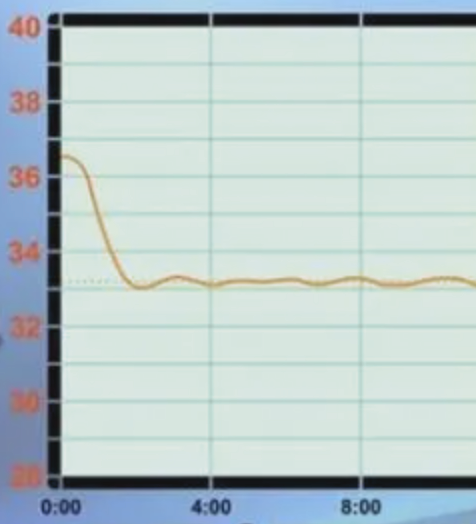
\includegraphics[width=0.6\textwidth]{./Figures/recorte-equipo.png}
	\caption{Evolución de la temperatura del paciente.}
	\label{fig:recorte-equipo}
\end{figure}

\newpage
\section{Contextos de uso del equipo}

Si bien se detalla el protocolo a seguir, y en muchos casos se tiene en cuenta, existen casos en los que no. En algunos tratamientos la temperatura objetivo es establecida en 32.5 ºC, y en otros fue establecida en otros valores, entre los 30 ºC y los 35 ºC. Además se dan situaciones en las que el paciente no está correctamente sedado en la incubadora. Esto produce que el equipo tarde más de lo usual en llevarlo al objetivo y que la oscilación de la temperatura del paciente sea mayor. También se da que se mueve al niño, y esto produce que en ese momento la temperatura diste del objetivo. Estos contextos se comparan en la tabla \ref{tab:contextos-uso}. 

\begin{table}[h]
	\centering
	\caption[Contextos de uso]{Comparación de contextos de uso.}
	\begin{tabular}{l c}  
		\toprule
		\textbf{Situación} 	 & \textbf{Consecuencia}  \\
		\midrule
		Temperatura objetivo distinta & Tratamiento no estándar e impreciso \\		
		Paciente que no está sedado  & Tratamiento impreciso  \\
		Se mueve al paciente & Tratamiento impreciso por un lapso de tiempo \\		
		\bottomrule
		\hline
	\end{tabular}
	\label{tab:contextos-uso}
\end{table}

Como se mencionó, estos contextos de uso reducen la eficiencia del funcionamiento del equipo. Esto genera una oportunidad para el nuevo modelo. Se espera que esta nueva herramienta tenga mayor robustez y se comporte mejor ante contextos diversos. Esto puede lograrse a partir de un aprendizaje sólido y de un conjunto de datos amplio. Además diversas estrategias pueden ser aplicadas para maximizar la robustez del modelo. Esto se comentará en el siguiente capítulo.

\section{Redes neuronales informadas por física}
En esta sección se describen conceptos generales de redes neuronales y el enfoque de redes informadas por física, que son los fundamentos el desarrollo de los modelos.

\newenvironment{conditions}
{\par\vspace{\abovedisplayskip}\noindent\begin{tabular}{>{$}l<{$} @{${}={}$} l}}
	{\end{tabular}\par\vspace{\belowdisplayskip}}

\subsection{Redes neuronales}
Para el desarrollo de este trabajo se utilizaron diversos algoritmos de inteligencia artificial, siendo las redes neuronales las que mejores resultados presentaron. 
Las redes neuronales artificiales (RNA) son modelos computacionales que se inspiran en el funcionamiento del cerebro humano. La unidad de procesamiento fundamental de las redes neuronales suele ser denominada perceptrón o neurona.  Este recibe un vector de señales de entrada $ x =(x_1, x_2, . . . , x_n) $, las cuales se multiplican por un vector de pesos $W = (w_1, w_2, . . . , w_n)$. Esto se resume en la siguiente suma $\sum_{i=1}^n x_i  w_i$
También se añade valor denominado sesgo, que es un término independiente cuyo fin es otorgar flexibilidad en el aprendizaje de conceptos.
Por último a la salida de cada perceptrón se le aplica una transformación no lineal, llamada función de activación $g(z)$.  En conclusión, la salida de cada neurona se expresa como \ref{eq:neurona}.

\begin{equation}
	\label{eq:neurona}
	\hat{y} = g(z) = \sum_{i=1}^n x_i  w_i + b
\end{equation}

Para este modelo la función de activación que mejores resultados otorgó es la tangente hiperbólica, definida como $tanh(x) = \frac{e^x - e^{-x}}{e^x + e^{-x}} = \frac{1 - e^{-2x}}{1 + e^{-2x}}$.

En particular en este trabajo se desarrollaron modelos de aprendizaje profundo, que son redes neuronales multicapa \citep{Goodfellow-et-al-2016}. Estas arquitecturas están compuestas por al menos 3 capas. La primera es denominada capa de entrada, que suele tener tantas neuronas como la longitud de los vectores de entrada. A ésta le sigue la capa oculta, y luego sigue una capa de salida, con tantas neuronas como la longitud del vector de salida del modelo.

El aprendizaje en estos modelos se da a partir de una función de entrenamiento cuyo objetivo es minimizar el error en las predicciones. Definida una función de error $L(\hat{y},y)$, el objetivo es minimizar su valor. En este caso se utilizó el entrenamiento por descenso del gradiente. En este algoritmo el error se reduce de forma iterativa buscando un mínimo en la función a través del gradiente. En cada iteración se calcula el siguiente punto en el espacio como una resta entre el punto actual y el gradiente en ese punto multiplicado por un factor de aprendizaje. Desde el punto de vista geométrico, al restar el gradiente lo que sucede es que se están modificando los pesos hacia la dirección donde crece la función, esto es, hacia algún mínimo, que puede ser local o global. Este proceso se repite hasta alcanzar un número máximo de iteraciones. En términos generales ésto se puede representar con la ecuación $p_{i+1} = p{i} - \gamma \nabla L(\hat{y},y)$. Esto se propaga para modificar los pesos de cada neurona mediante la técnica de \textit{back propagation } \citep{Goodfellow-et-al-2016}.

Este comportamiento se describe en la figura \ref{fig:gradient}. Se visualiza que para un punto $T_i$ se calcula al punto $T_{i+1}$ en la dirección geométrica del mínimo local.

\begin{figure}[htbp]
	\centering
	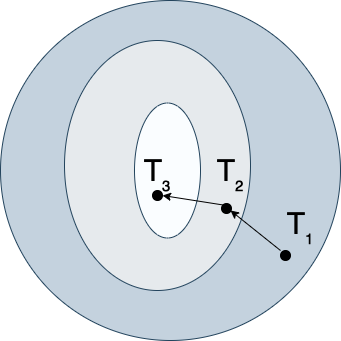
\includegraphics[width=0.5\textwidth]{./Figures/gradient.png}
	\caption{Ilustración del algoritmo de descenso del gradiente.}
	\label{fig:gradient}
\end{figure}

\subsection{Consideraciones físicas}
En principio, existe una temperatura mínima y máxima para el agua que circula en el equipo. El rango válido es entre 5 ºC y 40 ºC. Sin embargo en la práctica no es normal que el agua circule a temperaturas menores a 15 ºC por lo que podemos considerar como primer limitación física que la temperatura del agua esté entre los 15 ºC y los 40 ºC.  Por esto la misma respeta la expresión \ref{eq:umbrales_temperatura}.

\begin{equation}
	\label{eq:umbrales_temperatura}
	t : t >= 15 \circ \land  t <= 40 \circ
\end{equation}

Otra consideración es que se deben evitar en lo posible los cambios bruscos de temperatura. El algoritmo actual intenta generar cambios de 0,1 ºC. Si bien esto no es un requerimiento, las buenas prácticas en este tipo de tratamientos indican que la temperatura no cambie de forma brusca. Entonces, la bondad del modelo es inversamente proporcional a la magnitud del cambio de temperatura. Esto queda expresado en \ref{eq:bondad_vs_cambio_t}.

\begin{equation}
	\label{eq:bondad_vs_cambio_t}
	Bondad\propto \frac{1}{T_i - T_{i+1}}
\end{equation}

Dado que la respuesta del modelo es una temperatura a la que se debe calentar o enfriar el agua, se tiene en cuenta la energía necesaria para el cambio de temperatura a aplicar. Para esto se plantea en la ecuación \ref{eq:e_cambio_t} la energía requerida.

\begin{equation}
	\label{eq:e_cambio_t}
	E = m c \Delta T
\end{equation}

donde
\begin{conditions}
	m     &  masa del agua \\
	c     &  capacidad calorífica del agua \\   
	T &  temperatura
\end{conditions}

En términos generales, los modelos de inteligencia artificial vistos funcionan como sistemas de caja negra \citep{ML_methods}, es decir, modelos cuyo funcionamiento resulta muy difícil de explicar. Dadas las condiciones físicas del problema, se prefirió un enfoque de caja gris \citep{YANG2024121523}, que busca tener mayor control en su funcionamiento y por esto, una mejor capacidad para entender su comportamiento.
Para lograr esto se buscó incorporar las condiciones mencionadas al modelo. Se utilizó el enfoque de redes informadas por física \citep{cuomo2022scientificmachinelearningphysicsinformed}. Este tipo de redes se diseñó como una solución para los modelos de aprendizaje profundo diseñados para resolver problemas gobernados por principios físicos esenciales. En este paradigma se restringen las predicciones a soluciones coherentes con tales principios. Para esto incorporan en su aprendizaje los modelos físicos que gobiernan al problema. Esto proporciona una gran versatilidad ya que se tiene la capacidad de aprender de los datos y la de mantener las ecuaciones físicas que rigen en el problema. Para lograr esto, en este trabajo se definió una función de costo específica. Esta función tiene en consideración las ecuaciones vistas en esta sección y la función de error original, que es la diferencia entre la temperatura generada en el paciente y la objetivo. En el siguiente capítulo se explica como se diseñó esta solución.

En la figura \ref{fig:loss} se muestra un ejemplo de una función de error. El algoritmo de entrenamiento puede converger en algún mínimo local. Para este ejemplo, el mínimo de la sección mas clara de la gráfica es un mínimo que no cumple con las condiciones físicas. Siguiendo esta función para el entrenamiento, es posible que el modelo converja a la solución que no cumple las propiedades físicas del problema. 

\begin{figure}[htbp]
	\centering
	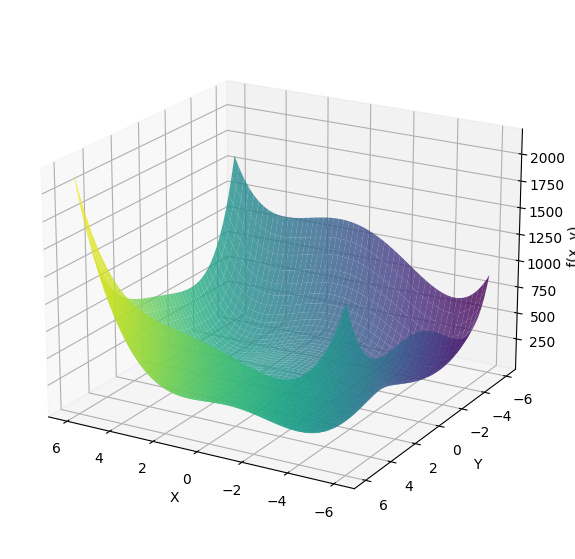
\includegraphics[width=0.6\textwidth]{./Figures/loss_example.png}
	\caption{Ejemplo de función de costo.}
	\label{fig:loss}
\end{figure}

Mediante redes informadas por física se puede modificar la función de costo, penalizando estas secciones, dejando como mínimos a los que cumplan con las propiedades. En la figura \ref{fig:modified-loss} se muestra un ejemplo como puede quedar la función de costo luego de incorporar los conceptos físicos.

\begin{figure}[htbp]
	\centering
	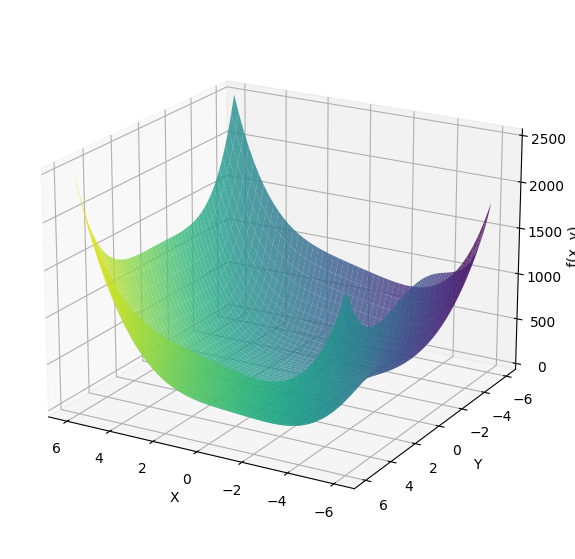
\includegraphics[width=0.6\textwidth]{./Figures/costo-modificada.png}
	\caption{Ejemplo de función de costo.}
	\label{fig:modified-loss}
\end{figure}

\section{Herramientas de software}
Como lenguaje de programación se utilizó Python \citep{python}. Este es un lenguaje de programación de alto nivel, interpretado, y multiparadigma. Cuenta con numerosas funciones propias del lenguaje que facilitan el desarrollo, y una amplia comunidad de soporte. Además es un lenguaje estándar en soluciones de inteligencia artificial.
También se utilizó Jupyter-Notebook \citep{jupyter}, que es un proyecto que facilita la programación interactiva. Permite dividir al código en celdas y ejecutar todas las sentencias que estén contenidas en una celda. 
Para el desarrollo de este trabajo se utilizó Visual Studio como entorno de desarrollo integrado. Este entorno permite desarrollar y ejecutar de forma amigable tanto archivos puros en Python como otros con extensión .ipynb, que son los que siguen el proyecto Jupyter-Notebook y el paradigma de ejecución por celdas. Esto permitió un desarrollo ágil de los modelos y los módulos necesarios.

Este trabajo se basó en herramientas de software útiles y de calidad comprobada en la industria por ser estándares. Para la manipulación de diversos objetos matemáticos se utilizó Numpy \citep{numpy}, que es una biblioteca potente que ofrece múltiples facilidades para éstas prácticas. 
Mediante Matplotlib \citep{matplotlib} se visualizaron gráficos que permiten entender mejor las relaciones entre los datos y las comparaciones realizadas. 
TensorFlow \citep{tensorflow} en general y Keras \citep{keras} en particular como frameworks para construir redes neuronales, debido a su potencia y a su flexibilidad para definir una función de costo específica y confiable.
Además se utilizó Scikit-Learn \citep{scikit-learn} como framework para implementar modelos de inteligencia artificial auxiliares y la realización de pruebas preliminares, como para segmentar datos y calcular meta datos.

En la figura \ref{fig:software} se muestra un diagrama que busca explicar las herramientas utilizadas y su relación. En el centro están los frameworks de desarrollo de modelos de inteligencia artificial, que son atravesados por herramientas trasversales como Numpy y Matplolib, y están contenidos en Python que es el lenguaje de programación utilizado.

\begin{figure}[htbp]
	\centering
	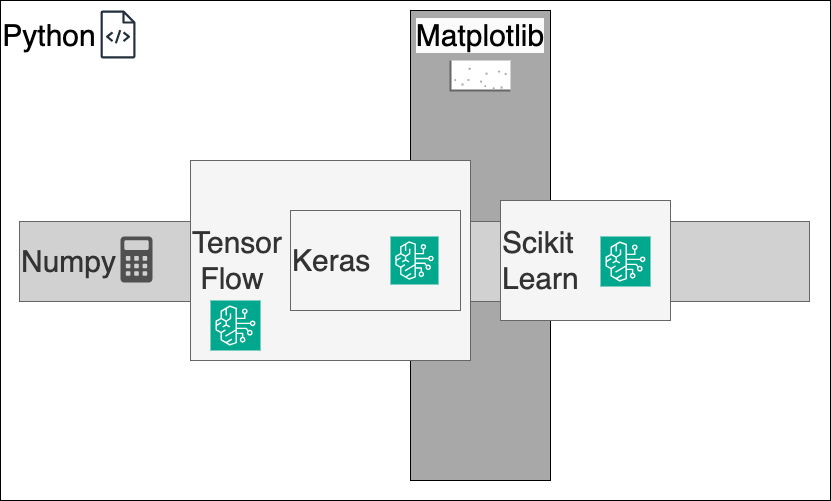
\includegraphics[width=1\textwidth]{./Figures/software.png}
	\caption{Diagrama de herramientas de software.}
	\label{fig:software}
\end{figure}
 
\chapter{Diseño e implementación} % Main chapter title

A continuación se describirá la solución implementada en el trabajo. Se mostrará la arquitectura utilizada, se comentará como fue el pre procesamiento y análisis de datos. También se analizarán los modelos de inteligencia artificial implementados, su arquitectura y particularidades. Por último se analizará el software integrador implementado.

\label{Chapter3} % Change X to a consecutive number; for referencing this chapter elsewhere, use \ref{ChapterX}

\definecolor{mygreen}{rgb}{0,0.6,0}
\definecolor{mygray}{rgb}{0.5,0.5,0.5}
\definecolor{mymauve}{rgb}{0.58,0,0.82}

%%%%%%%%%%%%%%%%%%%%%%%%%%%%%%%%%%%%%%%%%%%%%%%%%%%%%%%%%%%%%%%%%%%%%%%%%%%%%
% parámetros para configurar el formato del código en los entornos lstlisting
%%%%%%%%%%%%%%%%%%%%%%%%%%%%%%%%%%%%%%%%%%%%%%%%%%%%%%%%%%%%%%%%%%%%%%%%%%%%%
\lstset{ %
  backgroundcolor=\color{white},   % choose the background color; you must add \usepackage{color} or \usepackage{xcolor}
  basicstyle=\footnotesize,        % the size of the fonts that are used for the code
  breakatwhitespace=false,         % sets if automatic breaks should only happen at whitespace
  breaklines=true,                 % sets automatic line breaking
  captionpos=b,                    % sets the caption-position to bottom
  commentstyle=\color{mygreen},    % comment style
  deletekeywords={...},            % if you want to delete keywords from the given language
  %escapeinside={\%*}{*)},          % if you want to add LaTeX within your code
  %extendedchars=true,              % lets you use non-ASCII characters; for 8-bits encodings only, does not work with UTF-8
  %frame=single,	                % adds a frame around the code
  keepspaces=true,                 % keeps spaces in text, useful for keeping indentation of code (possibly needs columns=flexible)
  keywordstyle=\color{blue},       % keyword style
  language=[ANSI]C,                % the language of the code
  %otherkeywords={*,...},           % if you want to add more keywords to the set
  numbers=left,                    % where to put the line-numbers; possible values are (none, left, right)
  numbersep=5pt,                   % how far the line-numbers are from the code
  numberstyle=\tiny\color{mygray}, % the style that is used for the line-numbers
  rulecolor=\color{black},         % if not set, the frame-color may be changed on line-breaks within not-black text (e.g. comments (green here))
  showspaces=false,                % show spaces everywhere adding particular underscores; it overrides 'showstringspaces'
  showstringspaces=false,          % underline spaces within strings only
  showtabs=false,                  % show tabs within strings adding particular underscores
  stepnumber=1,                    % the step between two line-numbers. If it's 1, each line will be numbered
  stringstyle=\color{mymauve},     % string literal style
  tabsize=2,	                   % sets default tabsize to 2 spaces
  title=\lstname,                  % show the filename of files included with \lstinputlisting; also try caption instead of title
  morecomment=[s]{/*}{*/}
}


%----------------------------------------------------------------------------------------
%	SECTION 1
%----------------------------------------------------------------------------------------
\section{Arquitectura general del sistema}
 Sea $x$ el vector de datos de entrada, el objetivo es consturir un modelo cuya salida $y$ sea la temperatura del agua que debe circular por el equipo para que la temperatura del paciente se aproxime a la objetivo. Se definen tres valores protagonistas. Por un lado, el vector de entrada $x$, por otro lado la salida del modelo $y$, y por otro lado la temperatura a la que se lleva al paciente $y'$ si la temperatura del agua en el equipo es $y$.
Se define la función \ref{eq:f_x} como la relación entre $x$ y la temperatura del agua.

\begin{equation}
	\label{eq:f_x}
	y = f(x)
\end{equation}

La función \ref{eq:gx} es la relación entre $x'$ y la temperatura del paciente, siendo $x'$ el vector $x$ incluyendo como temperatura del agua a $y = f(x)$.

\begin{equation}
	\label{eq:gx}
	y' = g(x')
\end{equation}

Se define a la temperatura a la que se lleva al paciente como la composición de las funciones \ref{eq:f_x} y \ref{eq:gx} en la función \ref{eq:h_x}.

\begin{equation}
	\label{eq:h_x}
	y' = g(x \circ fx))
\end{equation}

A partir de estas funciones se ve que se deben representar dos relaciones. En primer lugar, dado un vector de datos de entrada $x$, cómo influye en la temperatura que tendrá el paciente en el siguiente periodo de tiempo, y en segundo lugar, dado un vector de datos de entrada $x$ cuál es la temperatura óptima del agua. Las dos relaciones son necesarias para el trabajo y ambas deben ser resueltas a partir de los datos. Para resolver estas relaciones se implementaron dos modelos de inteligencia artificial.

La arquitectura de los modelos implementados para representar estas funciones se muestra en la figura \ref{fig:architecture}. 

\vspace{1cm}

\begin{figure}[htbp]
	\centering
	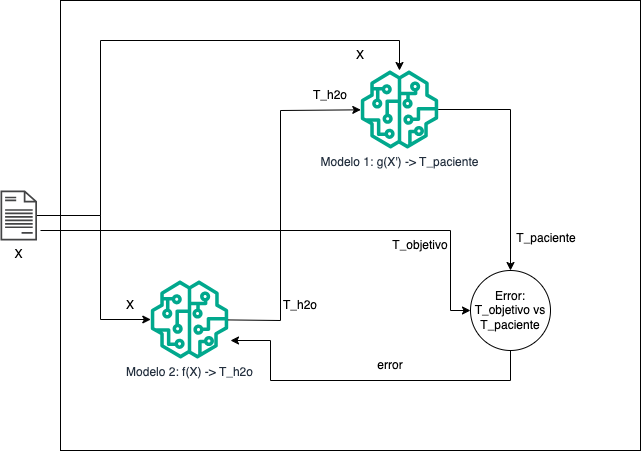
\includegraphics[width=1\textwidth]{./Figures/arquitectura_v2.png}
	\caption{Arquitectura de modelos del trabajo.}
	\label{fig:architecture}
\end{figure}

El modelo 1 implementa a la función \ref{eq:gx}. Fue entrenado en primera instancia a partir los datos del conjunto de datos recibido por el cliente. 
El modelo 2 implementa a la función \ref{eq:f_x}. Para entrenar este modelo la función de error no fue estándar. No existe, a priori, un vector $y$ con los valores certeros a los que el modelo 2 debe definir la temperatura del agua. Para entrenar al modelo 2 se debió utilizar al modelo 1, como se muestra en el círculo que representa a la función del error. El error se define como la diferencia entre la temperatura a la que se lleva al paciente con la salida del modelo y la objetivo. 
Se debe tener en cuenta que para definir a que temperatura se lleva al paciente dado un conjunto de datos se utiliza un modelo, que se entrenó a partir de los datos, y tiene un error en sus predicciones. 
Para el entrenamiento del modelo 2 no se deben modificar los pesos del modelo 1. Este último ya fue entrenado y debe utilizarse como caja negra. 
Se puede resolver este problema con un sólo modelo, cuyas últimas capas se entrenen en una etapa y sus primeras etapas, después. Pero este enfoque es mas complejo de implementar y ofrece menor claridad conceptual, por lo que se optó por la solución planteada.


\section{Análisis de los datos}
La empresa envío datos del tratamiento de casi 100 pacientes. Los datos estaban representados en tres formatos diferentes correspondientes a versiones del software del equipo, y en archivos de extensión .txt y .xlsx.
El equipo realiza una medición cada 15 minutos. Por esto cada tratamiento esta representado con dos secciones. La primera con información del paciente. De esta sección se consideraron el peso y la edad, ignorando cualquier dato identificatorio para resguardar la privacidad del paciente. La segunda consta de un conjunto con todas las mediciones realizadas por el equipo cada 15 minutos durante todo el tratamiento. 

Los datos considerados son los siguientes:
\begin{itemize}
	\item EDAD, en días.
	\item PESO, en gramos.
	\item FECHA INICIO, inicio del tratamiento.
	\item REG: Número de Registro.
	\item T\_SP: Temperatura objetivo.
	\item T\_H2O: Temperatura del agua que absorbe el calor del paciente.
	\item T\_PAC: Temperatura del paciente.
	\item MODO DE USO: Indica el modo de uso configurado.
	\item RAMPA\_HAB: Modo rampa habilitada, esto es influir en la temperatura del paciente para llevarla hacia el objetivo o hacia la normal, o deshabilitada, que consiste en mantener la temperatura estable.
	\item RAMPA\_SET: Indica la tasa de recalentamiento configurada para la función de rampa en °C / h.
	\item FECHA, de la medición.
\end{itemize}

La distribución de las temperaturas de los pacientes se muestran en la figura \ref{fig:pac}. La de las objetivo, en la figura \ref{fig:sp}, y la del peso de los pacientes en la imagen \ref{fig:peso}.
Se ven algunos valores extremos, como temperaturas de pacientes cercanas a los 0 ºC. Se verá en la siguiente sección el tratamiento que se da a estas anomalías. 

\begin{figure}[htbp]
\centering
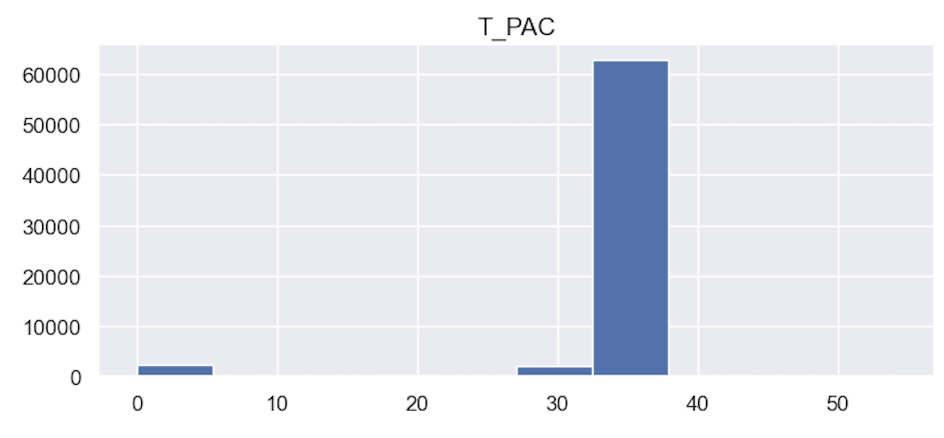
\includegraphics[width=0.5\textwidth]{./Figures/dist_t_pac.png}
\caption{Distribución de temperaturas de los pacientes.}
\label{fig:pac}
\end{figure}

\begin{figure}[htbp]
	\centering
	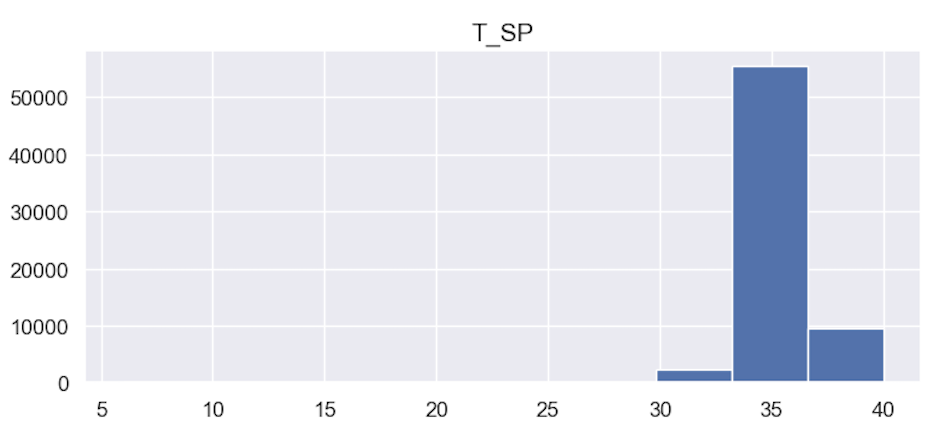
\includegraphics[width=0.5\textwidth]{./Figures/dist_sp.png}
	\caption{Distribución de temperaturas objetivo.}
	\label{fig:sp}
\end{figure}


\begin{figure}[htbp]
	\centering
	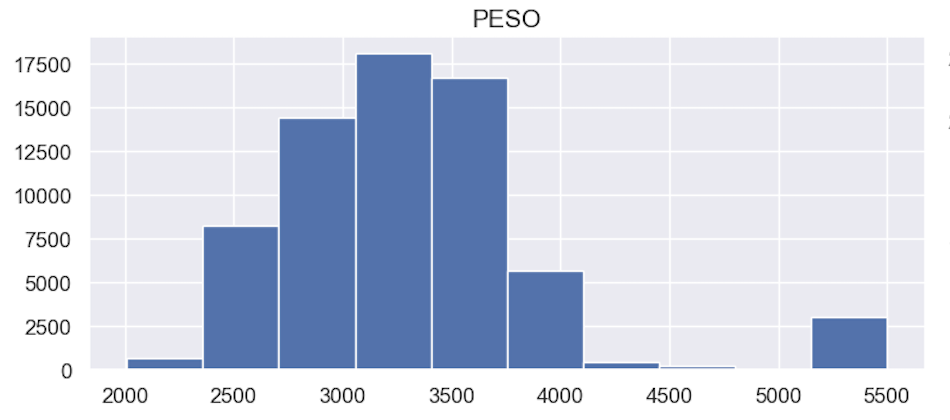
\includegraphics[width=0.9\textwidth]{./Figures/dist_peso.png}
	\caption{Distribución de pesos de los pacientes.}
	\label{fig:peso}
\end{figure}

En la figura \ref{fig:corr} se muestra la correlación entre las variables de los datos recibidos.
\begin{figure}[htbp]
	\centering
	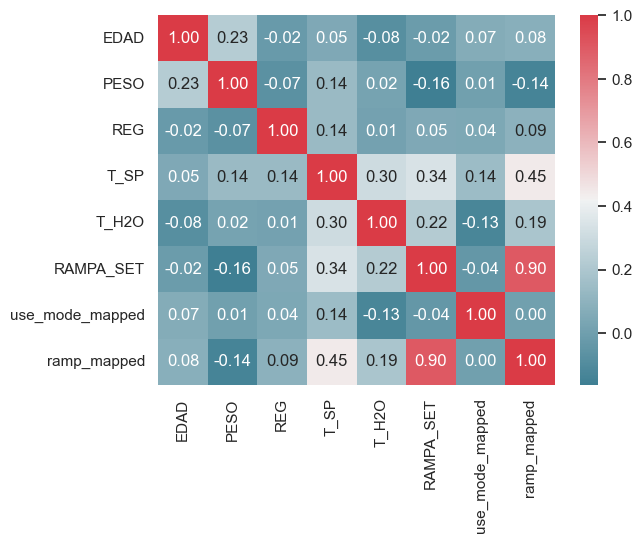
\includegraphics[width=0.9\textwidth]{./Figures/correlation.png}
	\caption{Correlación entre las variables.}
	\label{fig:corr}
\end{figure}

\section{Preprocesamiento de datos}

\include{Chapters/Chapter4} 
\include{Chapters/Chapter5} 

%----------------------------------------------------------------------------------------
%	CONTENIDO DE LA MEMORIA  - APÉNDICES
%----------------------------------------------------------------------------------------

\appendix % indicativo para indicarle a LaTeX los siguientes "capítulos" son apéndices

% Incluir los apéndices de la memoria como archivos separadas desde la carpeta Appendices
% Descomentar las líneas a medida que se escriben los apéndices

%\include{Appendices/AppendixA}
%\include{Appendices/AppendixB}
%\include{Appendices/AppendixC}

%----------------------------------------------------------------------------------------
%	BIBLIOGRAPHY
%----------------------------------------------------------------------------------------

\Urlmuskip=0mu plus 1mu\relax
\raggedright
\printbibliography[heading=bibintoc]

%----------------------------------------------------------------------------------------

\end{document}  
